\documentclass[10pt,a4paper]{ctexart}
\usepackage[margin=2cm]{geometry}
\usepackage{graphicx}
\usepackage{float}      % 支持 [H] 浮动体选项
\usepackage{hyperref}
\usepackage{amsmath}    % 提供方程环境
\usepackage{physics}    % 简化向量、微分算子语法
\newcommand{\myspace}[1]{\par\vspace{#1\baselineskip}} %自定义空一行
\usepackage{fancyhdr}
\usepackage{subcaption}
\pagestyle{fancy}
\fancyhf{}  % 清除所有页眉页脚
\fancyfoot[C]{\thepage}  % 在页脚中央设置页码
\renewcommand{\headrulewidth}{0pt}  % 去掉页眉横线
\renewcommand{\footrulewidth}{0pt}  % 去掉页脚横线

\usepackage{hyperref}
\hypersetup{
    colorlinks=true,
    linkcolor=blue,
    filecolor=magenta,      
    urlcolor=cyan,
    pdftitle={Overleaf Example},
    pdfpagemode=FullScreen,
    }

\usepackage{titlesec}

% 重新定义section格式
\titleformat{\section}
  {\normalfont\Large\bfseries}
  {\chinese{section}、}
  {0pt}
  {}

% 给出常用字号的自定义指令
\newcommand{\chuhao}{\fontsize{42pt}{48pt}\selectfont}
\newcommand{\xiaochu}{\fontsize{36pt}{42pt}\selectfont}
\newcommand{\xiaoer}{\fontsize{18pt}{21.6pt}\selectfont}
\newcommand{\sanhao}{\fontsize{16pt}{20pt}\selectfont}
\newcommand{\xiaosan}{\fontsize{15pt}{18pt}\selectfont}
\newcommand{\sihao}{\fontsize{14pt}{18pt}\selectfont}
\newcommand{\xiaosi}{\fontsize{12pt}{16pt}\selectfont}
\newcommand{\wuhao}{\fontsize{10.5pt}{12.6pt}\selectfont}

% 定义中文数字转换
\titleformat{\section}
  {\normalfont\Large\bfseries}
  {\zhnum{section}、}  % 使用\zhnum而不是\chinese
  {0pt}
  {}

% 标题设置
\title{\xiaochu\textbf{电子工程训练个人小结报告}}
\author{}
\date{}

\begin{document}

\vspace*{36pt} % 顶部空白

% 居中填写区域
\begin{center}
    
\includegraphics[width = 9cm]{figure/head.png}
    
    \xiaochu\textbf{电子工程训练个人小结报告}
    % 预留空白区域
    \vspace{13pt}
    \vspace{13pt}
    \vspace{13pt}
    \vspace{13pt}
    

    \sanhao\textbf{实验组号：\underline{\makebox[10cm]{ }}} \\[10pt]

    
    % 预留空白区域
    \myspace{6}
    
   \sihao\textbf{班级：\underline{\makebox[6cm]{}}} \\[10pt]
    \sihao\textbf{姓名：\underline{\makebox[6cm]{}}} \\[10pt]
    \sihao\textbf{学号：\underline{\makebox[6cm]{}}} \\[30pt]
    

    \vspace{18pt}
    
\end{center}

\newpage

\section{引言}

电子工程训练（甲）是本学期一门重要的专业实践课程。通过为期数周的动手操作与系统调试，我将《电子电路基础》等理论课程中的知识点，串联成了具体的、可触摸的工程实践。开课之初，面对电烙铁、电路板和各式仪器，我既感到陌生也充满好奇。随着课程推进，从最初的焊接练习，到智能插座的完整调试，再到智能小车的综合组装，我逐步克服了畏难情绪，建立起从原理图到实物的认知桥梁，并深刻体会到“纸上得来终觉浅，绝知此事要躬行”的道理。本小结旨在系统回顾课程中的实践经历、梳理收获与反思，并为后续学习指明方向。

\myspace{2}
\section{主要经历}

\subsection{项目一：焊接训练与电路调试}
本项目是工程实践的起点，主要训练手工焊接技能和常用仪器（万用表、示波器、信号源）的基本操作和电路的基本测试方法。

在焊接练习中，我最初遇到了“虚焊”问题。由于对焊点形成的热力学过程理解不足，我习惯性地快速点焊，导致焊锡未能充分浸润焊盘和引脚。
在观察到老师示范的“五步法”（准备、加热、送丝、移丝、移烙铁）后，我意识到“耐心加热”是关键。
在后续的贴片元件焊接中，我刻意放慢节奏，确保烙铁头同时接触焊盘和引脚，待焊锡熔化流动形成光滑凹面后再撤离。
当看到自己的焊点从最初的粗糙不均变得饱满光亮，并在评分中获得进步时，我感受到了扎实掌握基础技能的成就感。
\begin{figure}[H]
    \centering
    \begin{subfigure}[b]{0.32\textwidth}
        \centering
        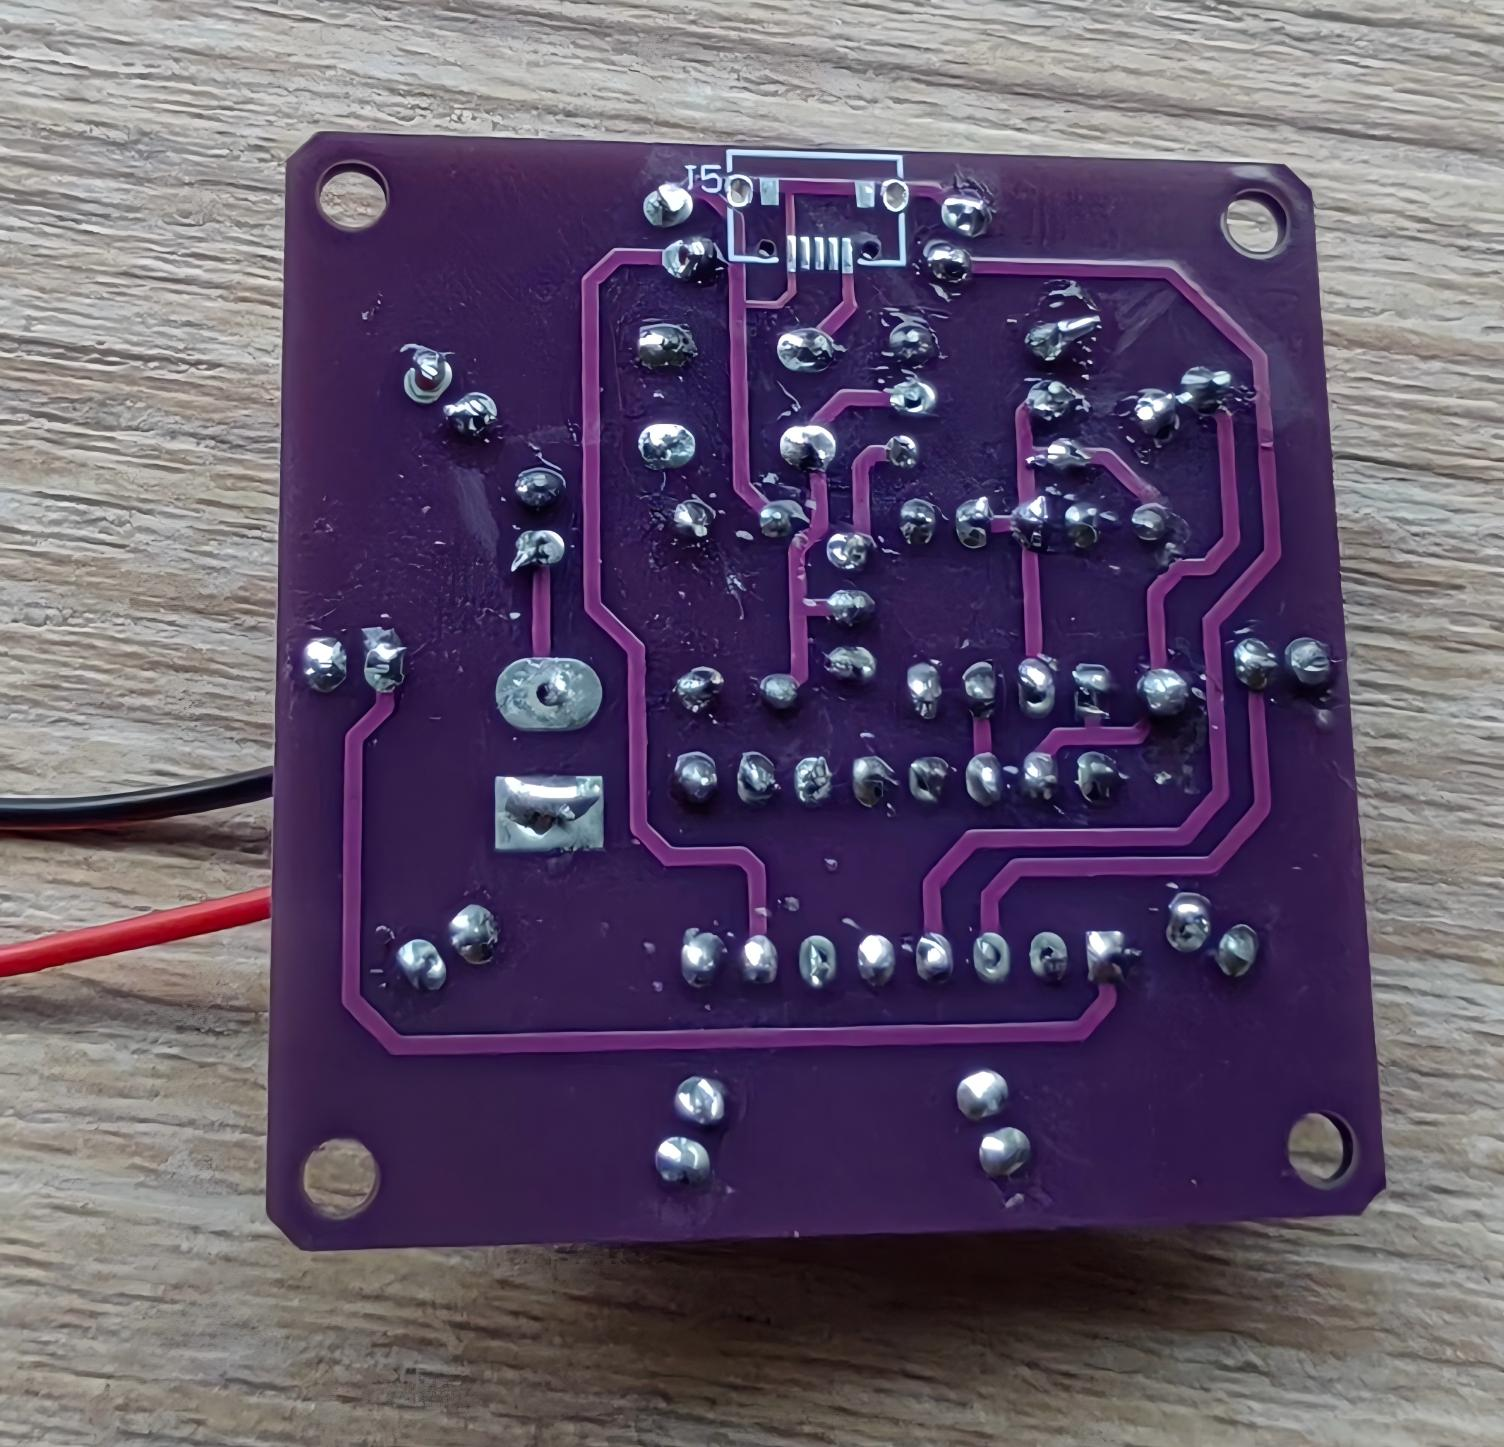
\includegraphics[width=\textwidth]{figure/幸运转盘电路板反面.jpg}
        \caption{幸运转盘电路板反面}
        \label{fig:cutoff_distort}
    \end{subfigure}
    \hfill

    \begin{subfigure}[b]{0.32\textwidth}
        \centering
        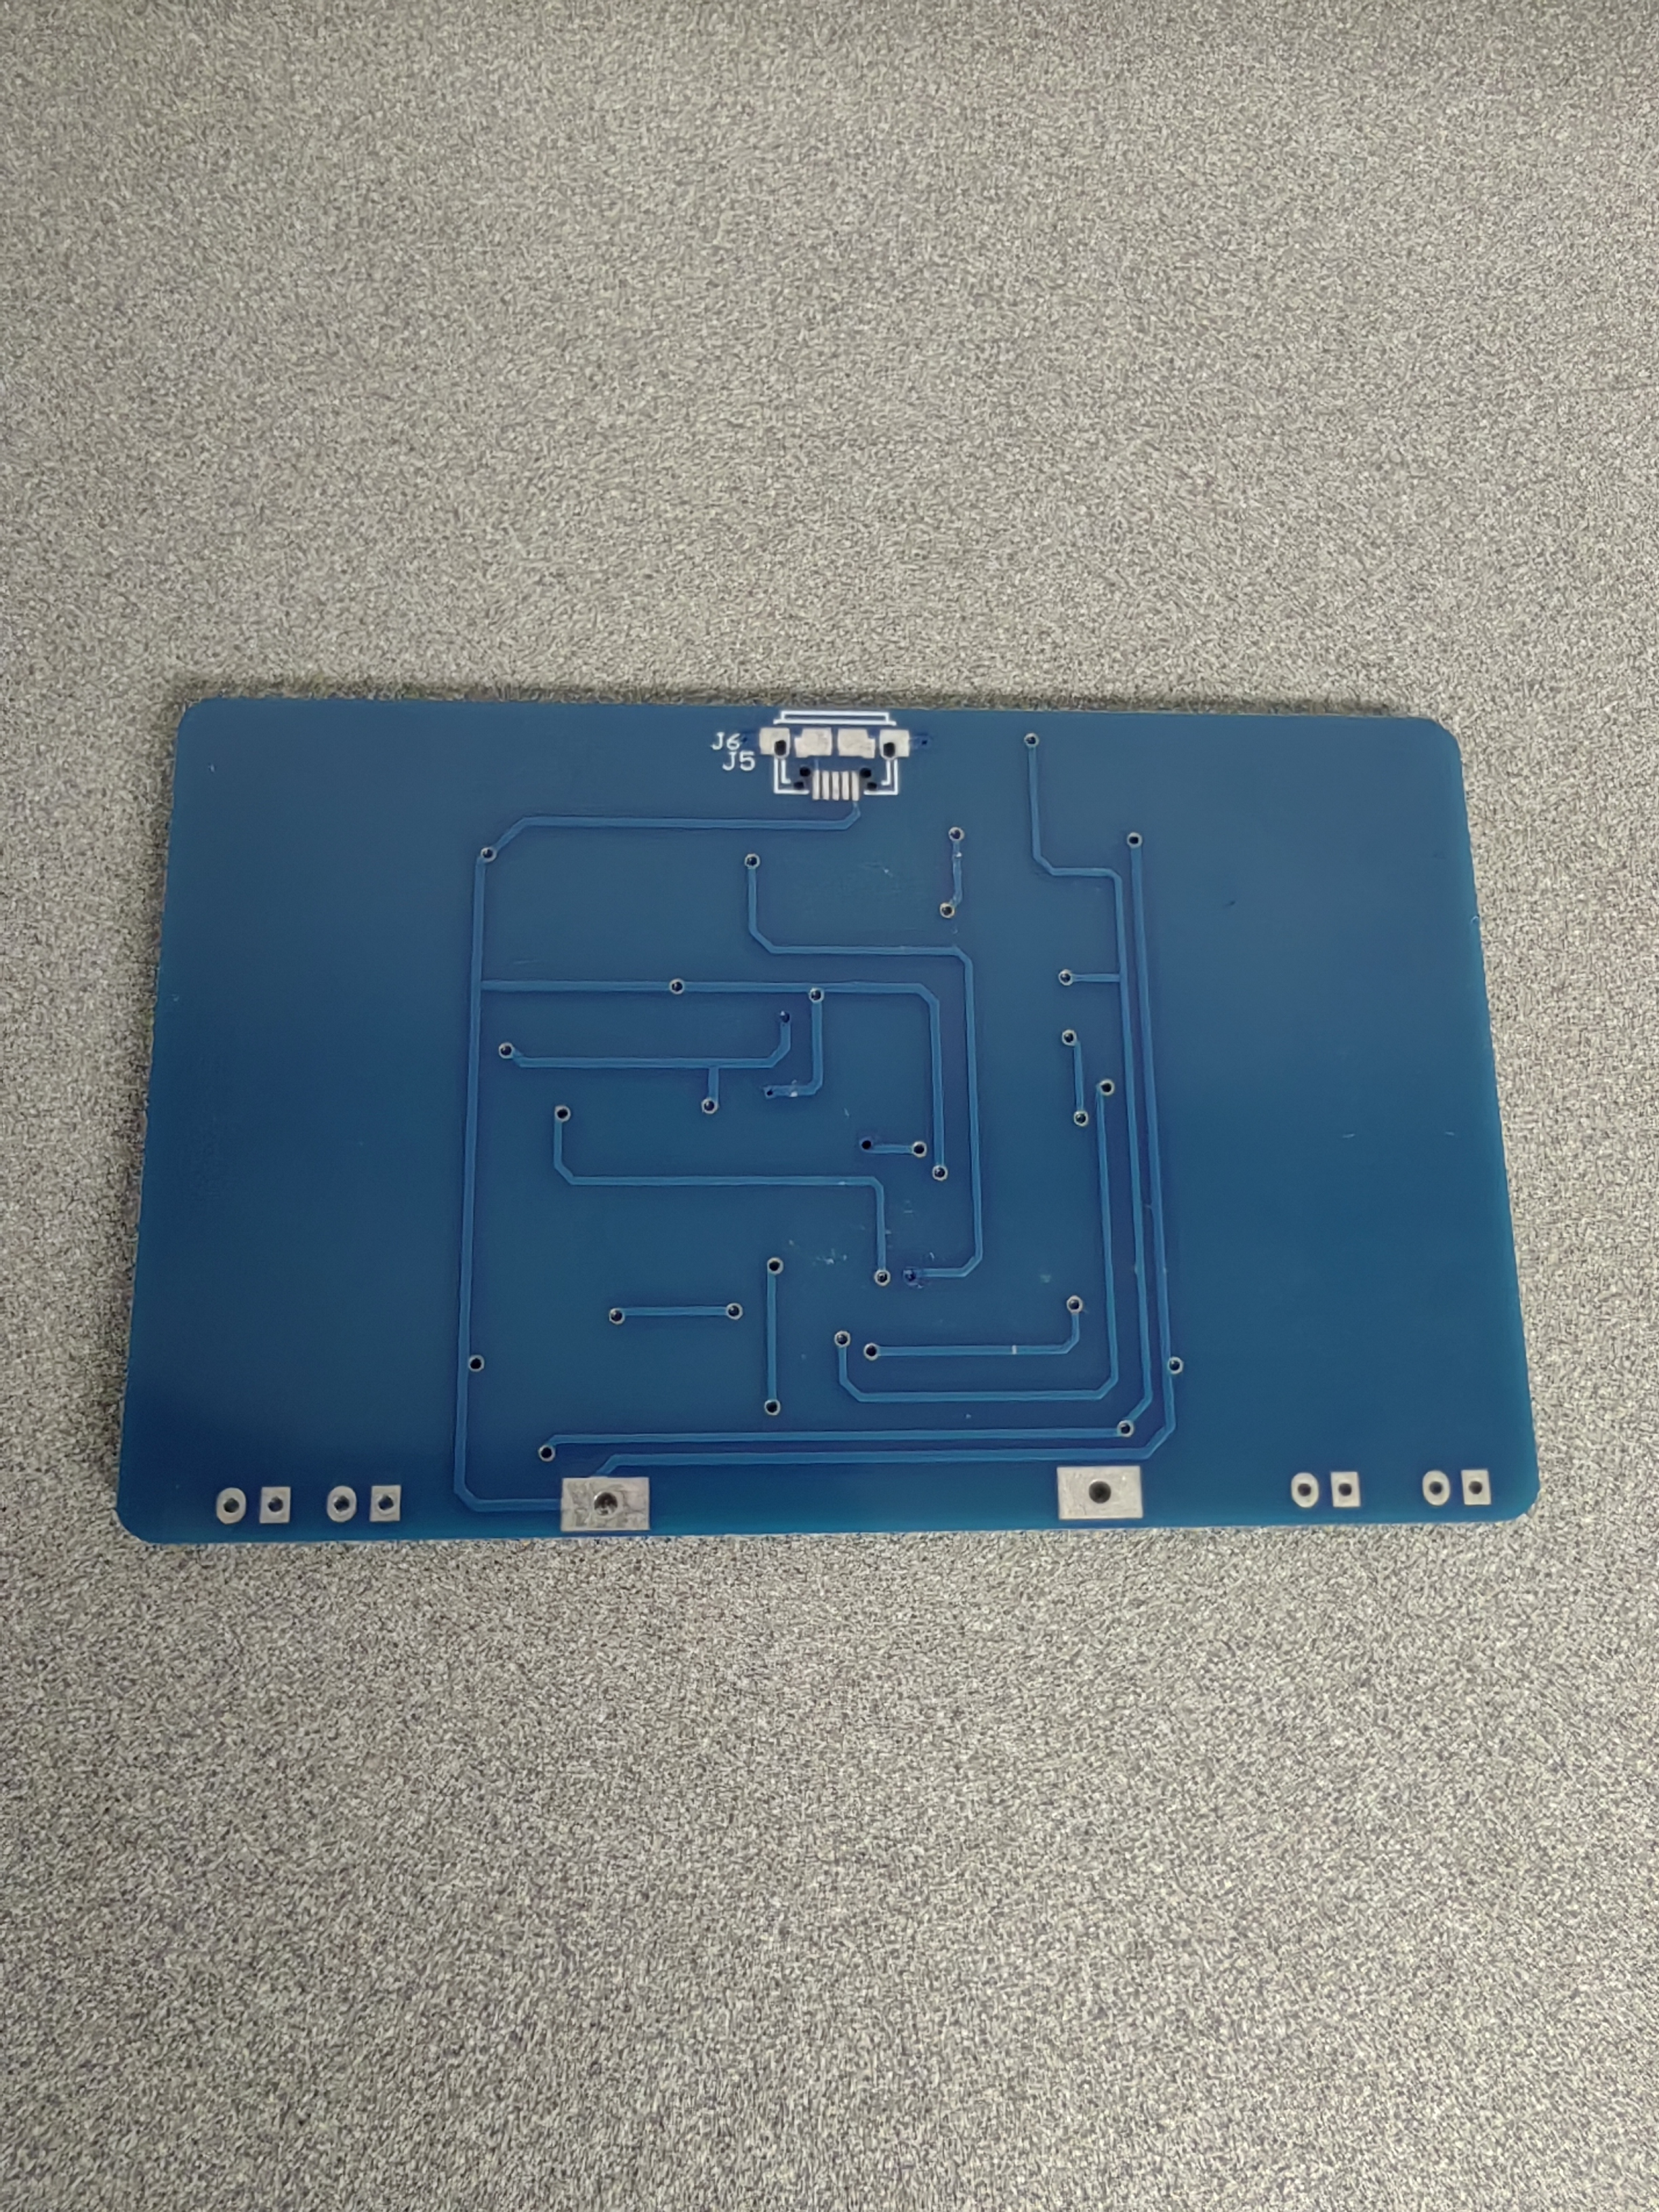
\includegraphics[width=\textwidth]{figure/贴片电路板反面.jpg}
        \caption{贴片电路板反面}
        \label{fig:sati_distort}
    \end{subfigure}
    \hfill

    \caption{两次焊接对比}
    \label{fig:contrast}
\end{figure}

仪器使用方面，最大的挑战来自示波器。在调试多波形信号发生器时，我需要观测并测量方波、三角波的频率与幅度。起初，由于触发模式（如边沿触发、自动/普通模式）和耦合方式设置不当，屏幕上的波形总是晃动或无法稳定。通过反复尝试和请教老师，我理解了“触发”的本质是让示波器在满足特定条件（如电压超过某一电平）时才进行波形捕捉与显示。

\subsection{项目二：智能插座的电装、调试、测试}
本项目是一个完整的电子系统实践，涵盖了电装、硬件调试、软硬件联调全流程。

在电装过程中，我负责根据BOM清单识别和分发元器件。这项工作看似简单，却让我深刻体会到理论与实践的鸿沟。例如，理论课上电容是一个抽象的符号C，而实物中却有着电解电容、瓷片电容等多种形态，且极性、封装各不相同。我曾误将一个小瓷片电容当作电解电容交给队友，导致焊错位置，幸好在通电前检查发现并纠正。这次教训让我明白，严谨细致、对照图纸核对每一个元件的型号、值和方向，是保证后续调试顺利的基础。
\begin{figure}[H]
    \centering
    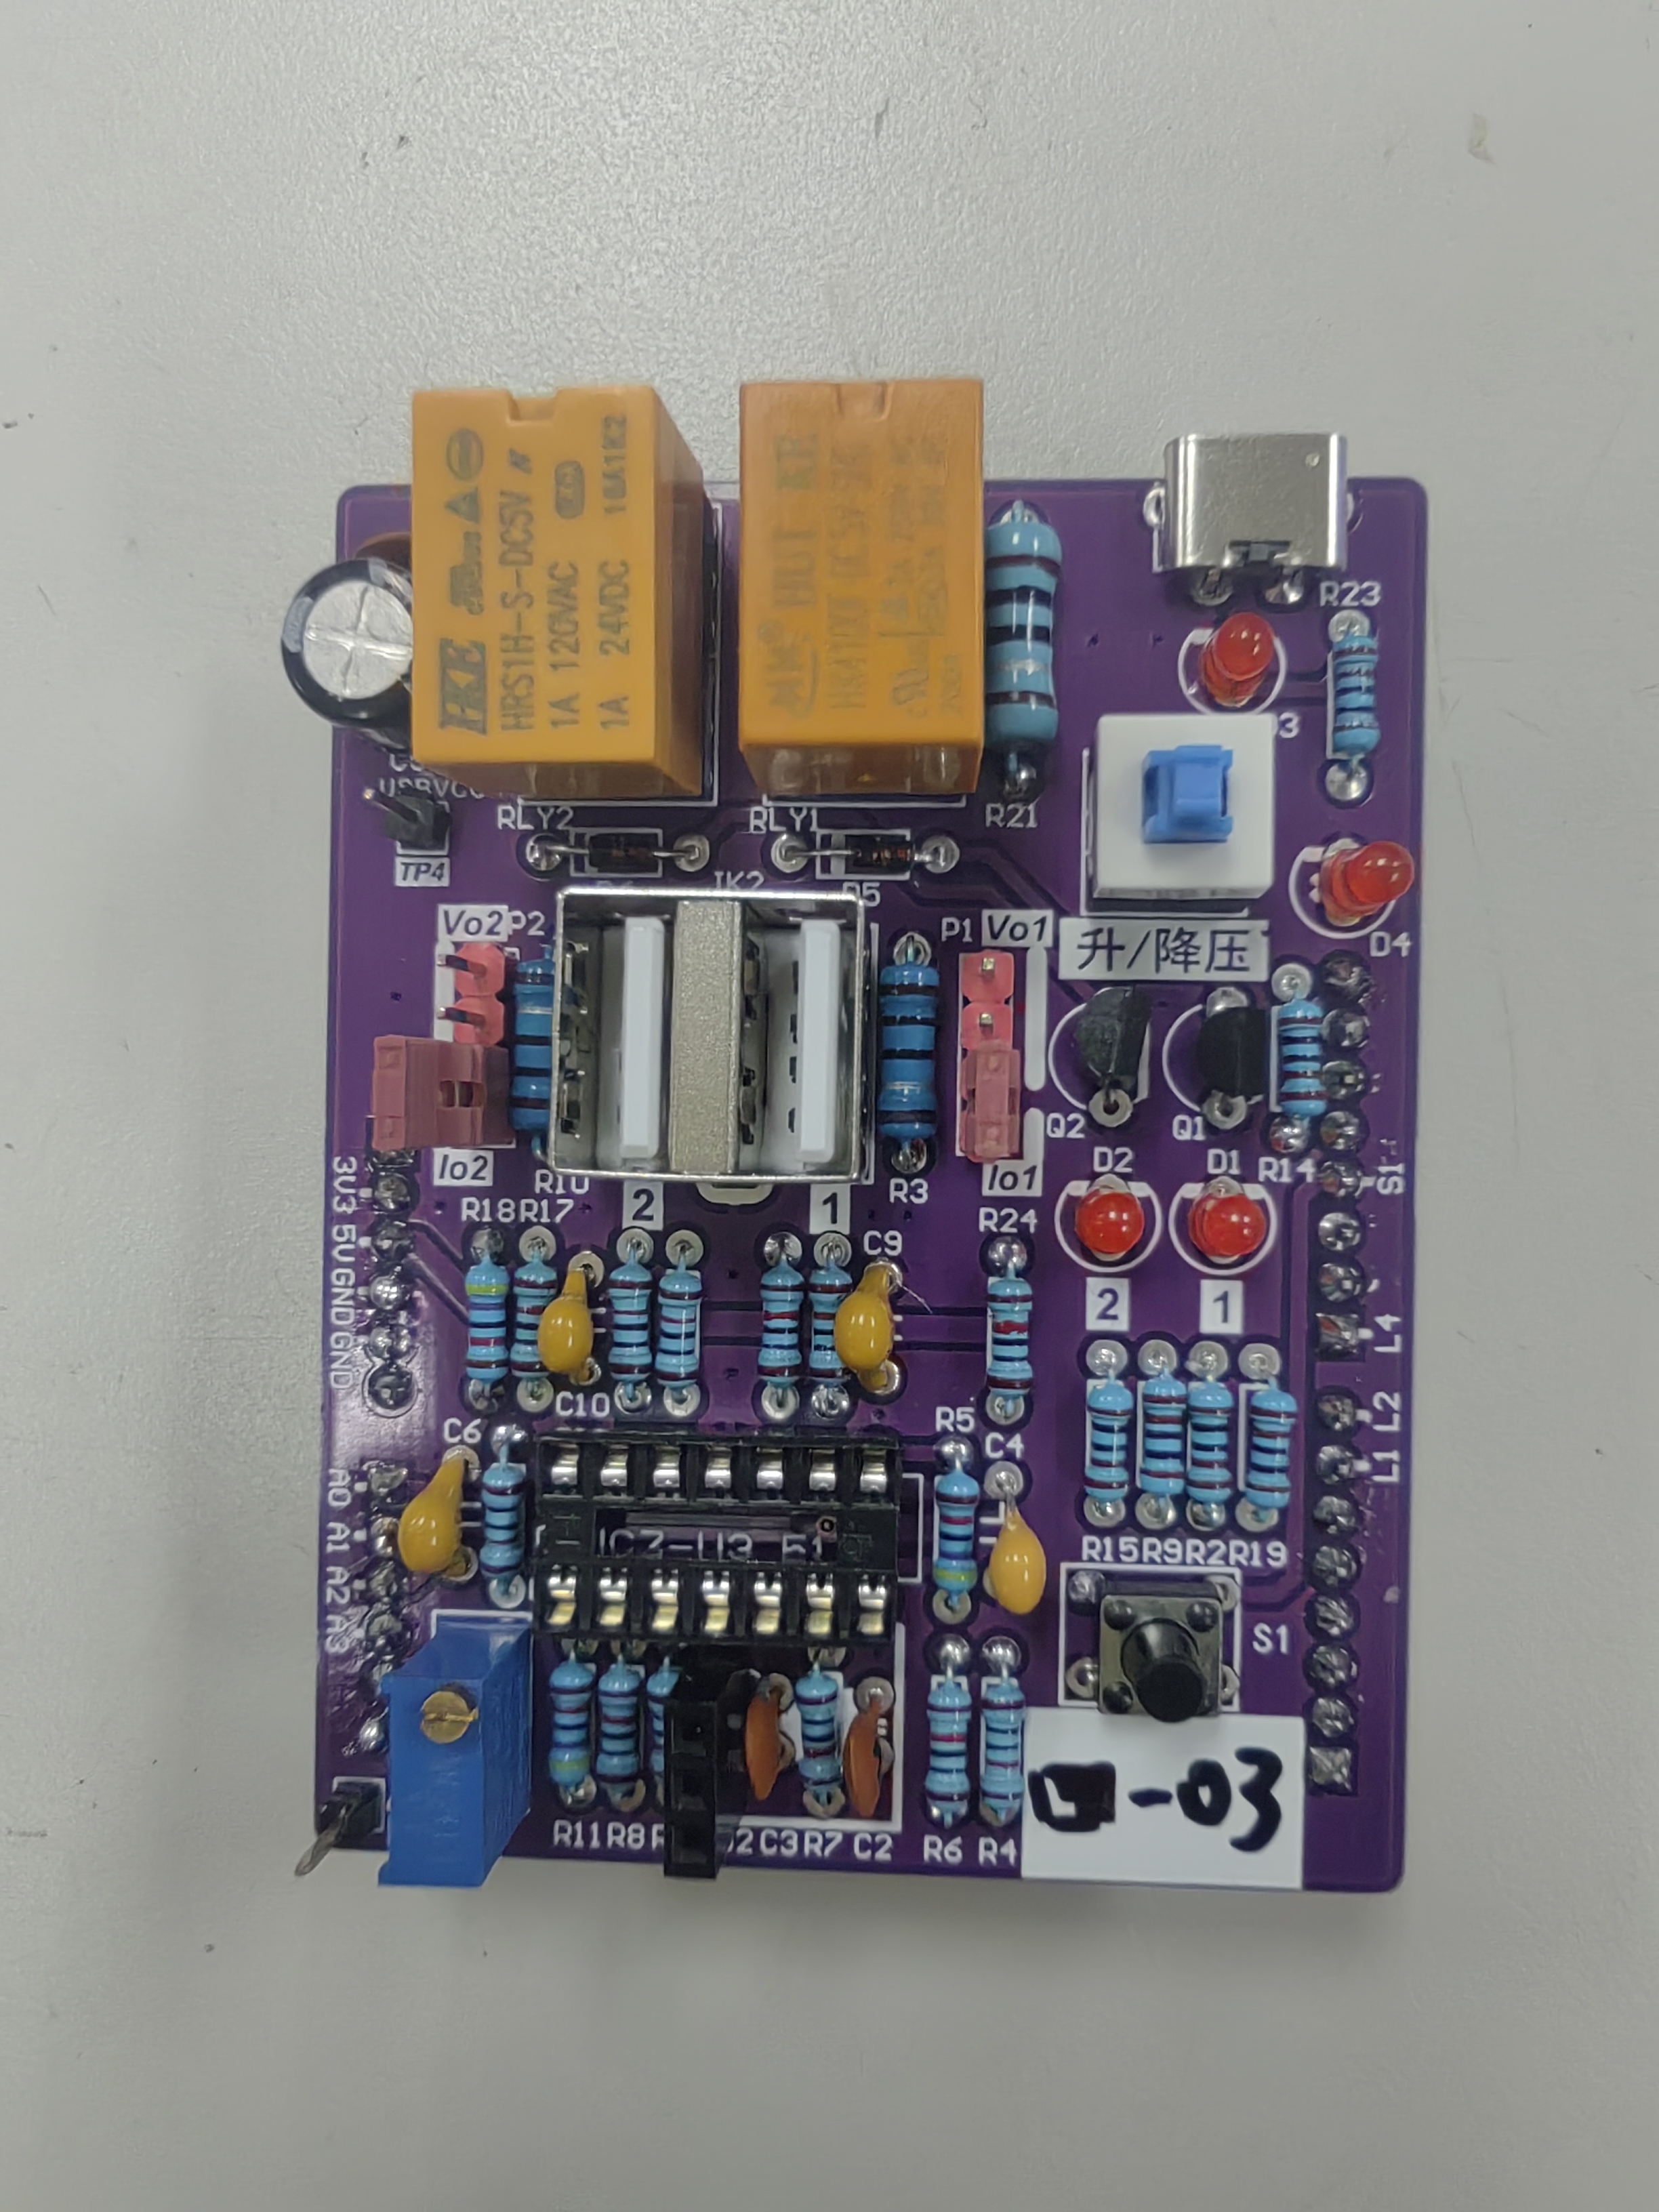
\includegraphics[width=0.4\textwidth, height=0.2\textheight]{figure/智能插座PCB.jpg}
    \caption{智能插座PCB}
    \label{fig:check}
\end{figure}
焊接完成后，我们进行了系统的硬件调试。其中最核心的是“标定”过程。这个过程不难，但是令我明白了标定的必要性和意义。
例如温度标定，我们需要通过调节可变电阻VR1，使LM35传感器读出的温度值与实际室温（25.7℃）一致。
我们最终将显示值校准至25.73℃，误差很小。
电流标定则更具挑战性，需要利用公式 \( I = k \times val + b \) 进行计算。
我们通过测量两组实际电流与采样值，求解出标定系数，并将公式写入程序。
修改后，在10个测量点的检验中，电流显示误差被控制在3\%以内。
这个过程让我认识到，由于元器件参数的离散性和电路的非理想性，任何测量系统都需要经过严谨的标定，才能获得可信的数据。而不应盲目相信未标定的读数。


调试与测试时队友操作电路，我思考并指示电路测试点、测量数据，读数并记录。智能插座在测试时第一次遇到了软硬结合的问题，需要我们设计代码来实现附加功能。
我们选择了“温度控制风扇启停”的联调任务。在理解程序框架后，我们添加了温度判断逻辑：当读取的温度超过设定阈值（28.0℃）时，程序发送高电平电压打开风扇插座；当温度低于阈值时，则发送低电平关闭风扇。调试中，我们用手触碰传感器模拟升温，成功实现了风扇的自动启停控制。这一任务虽小，却是我第一次亲手实现软硬件结合的任务，让我对嵌入式系统的工作原理有了最直观的认识。
\begin{figure}[H]
    \centering
    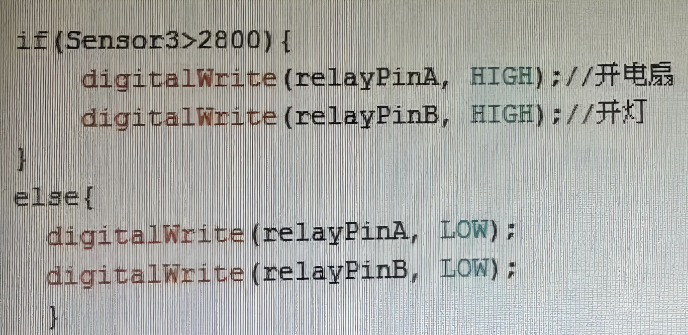
\includegraphics[width=0.4\textwidth]{figure/code.png}
    \caption{智能插座软件代码片段}
    \label{fig:smart_socket}
\end{figure}
项目后期的系统测试（如定时开关、过流保护）也让我了解到，一个成熟的产品需要经过反复的功能与边界测试。

虽然任务不难，但是感受到利用软件控制硬件的乐趣。通过编写代码，我们可以实现对硬件的智能控制，使其具备更多功能和更高的灵活性。这种软硬结合的设计思路让我对电子工程有了更深的理解，也激发了我对编程和电子设计的兴趣。

\subsection{项目三：智能小车的组装与调试}
智能小车项目是一个涉及机械、电子、软件的综合系统实践。项目要求我们完成从机械结构组装、传感器接线、到软件参数配置与功能联调的全过程。成功组装后的小车应具备语音控制、超声波避障、红外循迹及视频监控等基础功能，最终目标是通过视觉识别自动寻找并抓取指定颜色的小球。

本项目最大的特点在于参数调试的自主性与系统性。我们需要独立探索并设置云台舵机的运动范围、机械臂各关节的初始角度、摄像头颜色识别的阈值与范围等一系列参数。相比前两个项目，遇到的困难更为复杂多样。

首要挑战是机械与云台的空间协调。初期安装时，我们未充分考虑机械臂抓取时的运动轨迹，导致机械臂可能碰撞到云台摄像头。我们通过重新调整摄像头的安装位置与俯仰角度，为机械臂留出了安全的操作空间。

其次是小球识别系统的参数调试。小车的颜色识别极易受环境中其他物品影响，且小球初始位置可能较远。我们通过多次采样，反复调整最小识别半径，最终找到了能稳定识别小球的参数。
 
这个项目让我深刻体会到，一个复杂的机电一体化系统，其成功运行依赖于机械、硬件、软件参数之间精密的配合与大量的调试工作，任何环节的微小偏差都可能导致整体功能失效。
\begin{figure}[H]
    \centering
    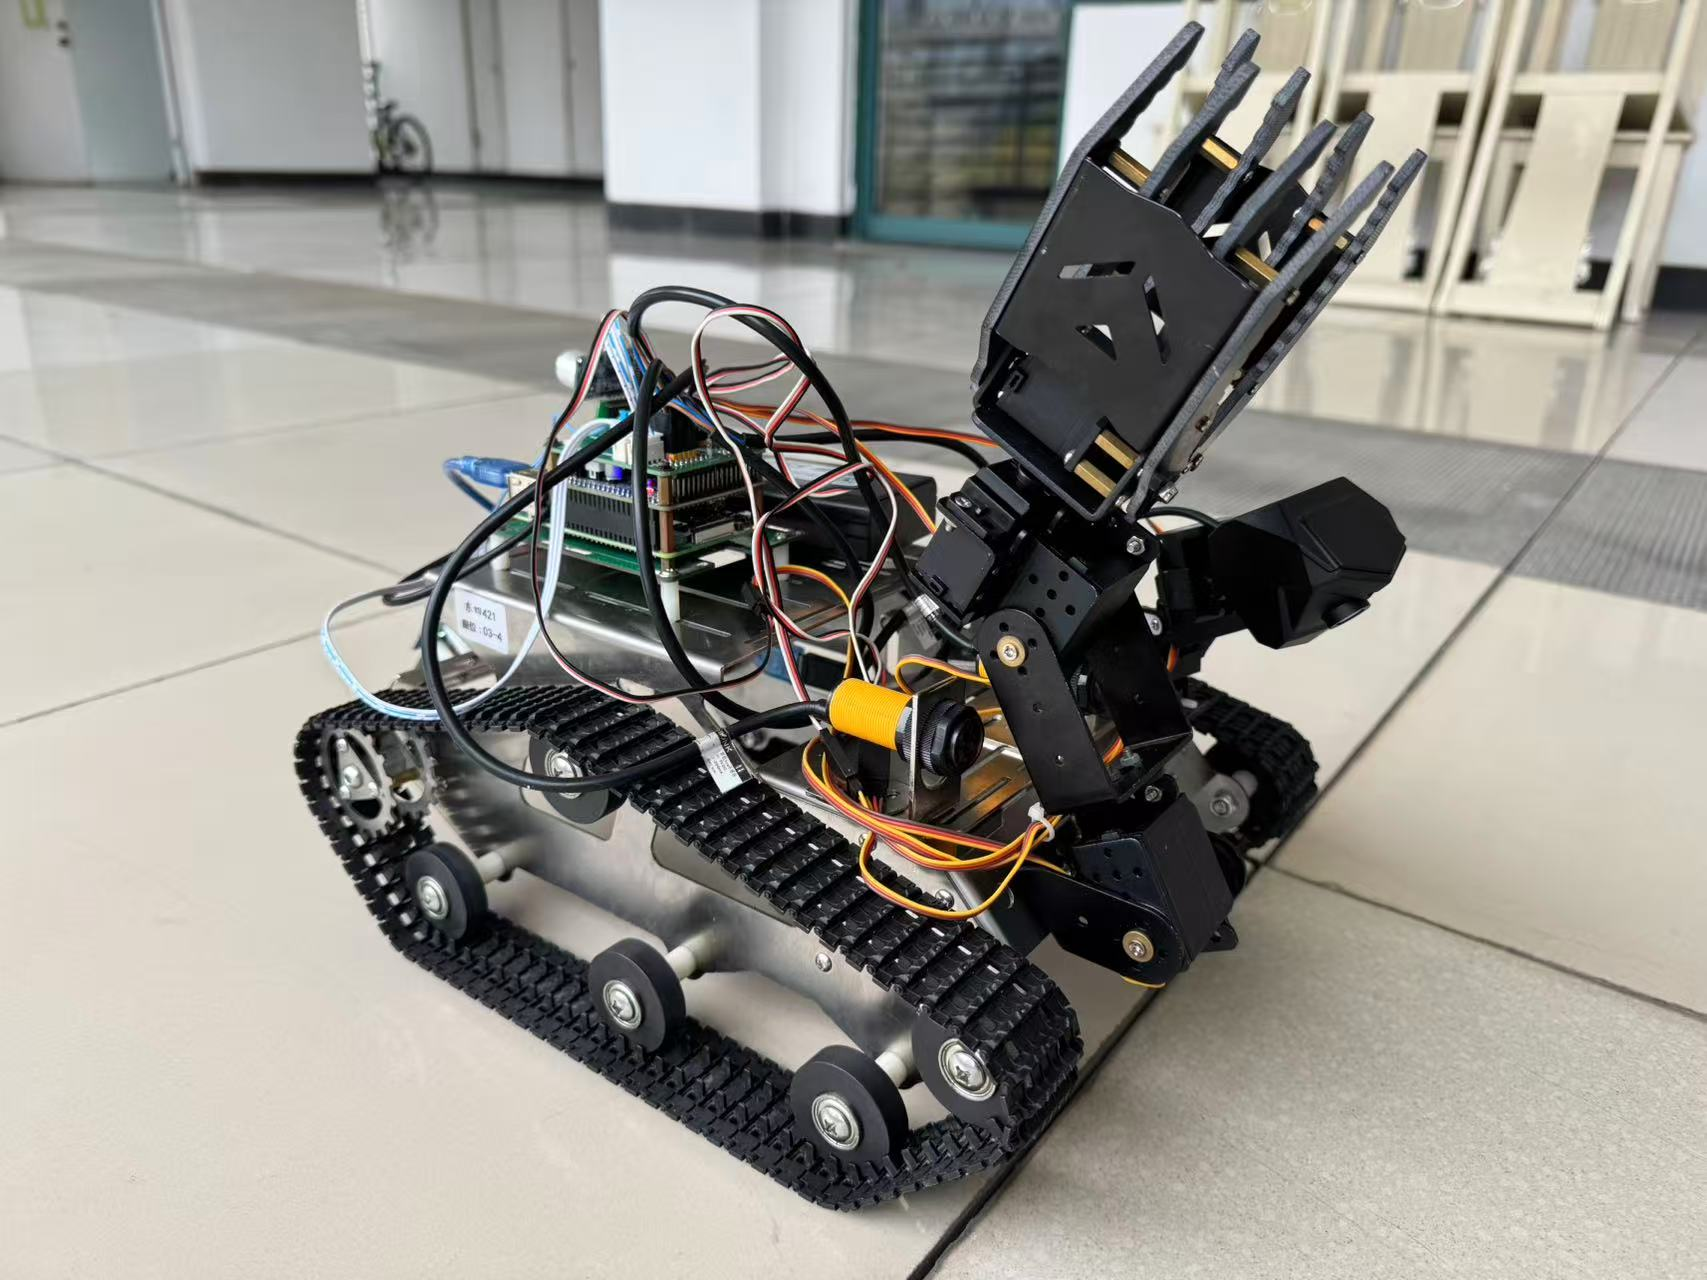
\includegraphics[width=0.5\textwidth]{figure/car.jpg}
    \caption{智能小车实物图}
    \label{fig:car}
\end{figure}
\section{收获与成长}
通过本课程的实践，我获得了多方面的提升：

首先，我对一个完整电子工程项目的开发流程建立了清晰的认识，从方案设计、元器件选型、电路焊接、系统调试到功能测试与优化，亲身体验了各环节的工作内容与规范要求。其次，我的实践操作能力得到了切实锻炼，掌握了手工焊接、仪器使用和电路调试的基本技能，并学会了面对故障时系统分析、逐级排查的解决方法。

尤为重要的是，我初步理解了软硬件协同工作的原理。在智能插座和小车的调试中，我通过修改程序代码实现了对硬件的控制，这让我对“软件定义硬件功能”有了直观体会。虽然项目的主电路由老师设计，但在老师讲解设计思路以及我们进行装配、测试的过程中，我学习到了如何从系统层面考虑功能的实现、电路的稳定性与安全性等实际问题。

总的来说，课程极大地培养了我对电子工程专业的兴趣。亲手将零散的元器件逐步组装、调试成一个能够可靠工作的完整系统，这个过程充满了探索的挑战与成功的乐趣，也让我更加坚定了在该领域继续学习与深造的决心。
\section{展望未来}
通过本课程的学习，我对电子工程领域有了更具体和深入的认识。未来，我希望能在以下方面继续深化：一是系统性地巩固和拓展模拟电路、数字电路以及嵌入式系统方面的理论知识；二是积极寻求并参与更多综合性的实践项目，在真实的工程环境中锻炼技术应用能力。我了解到学校在下学期将组织电子设计竞赛的相关培训，我计划报名参加，希望通过更具挑战性的项目，进一步提升电路设计、系统调试以及团队协作等方面的综合能力。

此外，回顾整个课程，我仍存在以下不足：首先，理论知识储备仍有欠缺，在调试电路时，对反馈、偏置等细节理解不够深入，对于电路没有直观的认识与理解。其次，在时间管理上，特别是在小车调试后期，由于对困难预估不足，导致部分调试任务时间紧张。最后，在团队沟通中，有时未能将自己的想法清晰表达，或未能完全理解队友的意图，未来需要加强主动沟通与复述确认。
\section{结语}
衷心感谢电子工程训练课程的所有指导老师和实验室老师的辛勤付出与耐心指导。老师们不仅传授了知识与技能，更以身作则展示了严谨求是的工程精神。同时，也感谢我的队友在整个过程中的紧密合作与互相支持。这段充满挑战与乐趣的实践经历，是我大学生活中浓墨重彩的一笔，它为我打开了电子工程实践的大门，必将激励我在未来的科技道路上不断探索。

\newpage


\end{document}